\documentclass[11pt,a4paper]{article}
\usepackage[margin=2.5cm]{geometry}
\usepackage[utf8]{inputenc}
\usepackage[T1]{fontenc}
\usepackage{hyperref}
\renewcommand{\familydefault}{\sfdefault}
\usepackage{helvet}
\pagestyle{empty}
\usepackage[kerning=true]{microtype}
\usepackage{parskip}
\usepackage{sansmath}
\usepackage[font={small, bf}]{caption}
\usepackage[font={small}]{subcaption}
\usepackage{graphicx}
\usepackage{multicol}
\setlength{\abovecaptionskip}{0pt}
\setlength{\floatsep}{10pt}
\setlength{\textfloatsep}{0pt}
\setlength{\intextsep}{0pt}
\setlength{\belowcaptionskip}{0pt}
\setlength{\parindent}{5ex}
\setlength{\parskip}{0pt}
% Feel free to use additional packages for glosses, figures, whatnot.

% The next bit is for reserving sufficient space for authors,
% affiliations, and e-mail address.  No need to change for initial
% anonymous version.  For the final version, replace the
% \toggletrue{anonymous} with \togglefalse{anonymous} to de-anonymize.
\usepackage{etoolbox}
\newtoggle{anonymous}
\togglefalse{anonymous}

\renewcommand{\title}[1]{\textbf{#1}\\}
\newcommand{\authors}[1]{\iftoggle{anonymous}{\phantom{#1}}{#1}\\}
\newcommand{\email}[1]{\iftoggle{anonymous}{\phantom{#1}}{#1}}

\begin{document}

% First page:

% Insert title, authors, affiliations, and e-mail address in the next three lines:

\title{A-maze of Natural Stories: Texts are comprehensible using the Maze task}
\authors{Veronica Boyce (MIT/Stanford), Roger Levy (MIT)} %TODO, check what affiliation I have at conference time
\email{vboyce@stanford.edu}
\newline
%
% Here goes the main text of your abstract:
%Comment: I feel like you could make a bigger deal of the current-word previous-word / RT correlation. Given how there are spillover effects for SPR and also for eye-tracking (if I’m not mistaken), it’s crazy that the relationship between RT/Surprisal for the previous word is basically flat, when it comes to Maze!
%Comment: I’m confused with Table 1: Doesn’t length have a bigger effect size than surprisal? On a related note: does it matter which has a bigger effect? Why is it important to say that surprisal has a bigger effect, compared to just a robust, significant effect?

A-maze is a new method for measuring incremental sentence processing that can localize slowdowns related to syntactic ambiguities (Boyce et al. 2020; Sloggett et al. 2020). We test A-maze on the Natural Stories corpus (Futrell et al. 2017) and find that people can comprehend what they read during the Maze task. Moreover, the Maze task yields useable reaction time data with word predictability effects that are linear in the surprisal of the current word, with little spillover effect from the surprisal of the previous word. 

The Maze task (Forster et al. 2009; Witzel et al. 2012) is an incremental processing method where participants read a sentence word by word  (Figure~1). For each word position, participants see two words, one of which is the next word in the sentence and one of which is a distractor. Participants press a key to indicate which word continues the sentence; the time between key presses (reaction time, or RT) is the dependent measure.  Traditionally, when a participant makes a mistake, the sentence stops and they move on to the next item. In order to present coherent texts, we instead have participants correct their mistakes (Figure~1). When a participant makes a mistake, they see an error message and must press the correct key to continue with the sentence. This way, participants see all the content and can follow the story, allowing us to test multi-sentence materials.

The Natural Stories Corpus consists of 10 passages ($\sim$1000 words each) with 6 comprehension questions per passage (Futrell et al. 2017). We used the A-maze framework from Boyce et al. (2020) and the language model from Gulordava et al. (2018) to generate distractor words for the texts. We recruited 100 participants from Amazon Mechanical Turk; each participant read one passage in the Maze task and answered the corresponding comprehension questions. 

We exclude 5 participants who do not report being native English speakers. Participants clustered into those who appear to randomly press keys to get through the task quickly and those who do the task more slowly and accurately (Figure~2); we exclude participants with less than 80\% accuracy from analyses. Task accuracy is correlated with performance on the comprehension questions ($r^2=.47$); of the 63 participants who had at least 80\% accuracy on the Maze task, 50 got 5 or 6 of the 6 comprehension questions correct (Figure~4). People can understand and remember what they read while doing the Maze task successfully.

We also investigated the relationship between a word's predictability and its RT. We fit Bayesian regression models using suprisal, frequency, length, and surprisal:length and frequency:length interactions at both the current and previous word as predictors of RT (see Table~1 for details). We use 3 models for surprisals: a Kneser-Ney smoothed 5-gram model, a recurrent neural network model (GRNN) from Gulordava et al. (2018), and a transformer model (TXL) from Dai et al. (2019). Across all models, we see large effects of current word surprisal and length, which noticeably exceed effects of previous word predictors (Table~1). We see minimal to no frequency effects (consistent with Shain 2019). We also fit GAMs to look at the shape of the relationship between surprisal and RT; we find a linear relationship between RT and current word surprisal and no relationship with previous word surprisal (Figure~3). The linear relationship matches known effects from eye-tracking and self-paced reading (Smith \& Levy 2013), but the lack of spillover indicates a potential advantage of Maze over eye-tracking and self-paced reading.


In summary, we provide an adaptation of the Maze task for long naturalistic texts, and show that participants can comprehend what they read during A-maze. Additionally, we find robust, localized surprisal effects, supporting Forster et al.'s (2009) argument that Maze forces highly incremental processing. Overall, this suggests that A-maze is a versatile alternative to eye-tracking and self-paced reading. 

Our code and data are available at [link to repo redacted for anonymity]. 

%It’s worth thinking about “why should AMLaP attendees care about this work?” and building an answer to that into the abstract.  Minimally, the work shows
%
%- Maze is really a flexible method
%- you can have people read naturalistic text passages with Maze, they can understand the passages and you wind up with usable data
%- word predictability effects in Maze are linear in surprisal, as they are with SPR and eye tracking
%- potentially unlike SPR or eye tracking, surprisal seems to be far more important than word length or word frequency as a determinant of processing time in Maze (see comments/questions below about the model)
%- also potentially unlike SPR or eye tracking, there isn’t much spillover in Maze for word predictability effects (though there is a little for word length).  All this seems to support Forster et al. 2009’s argument that Maze “forces highly incremental processing”.

\newpage
\begin{figure}
	\begin{minipage}{.5\textwidth}
		\captionof{figure}{Maze with Error Correction}
		{\center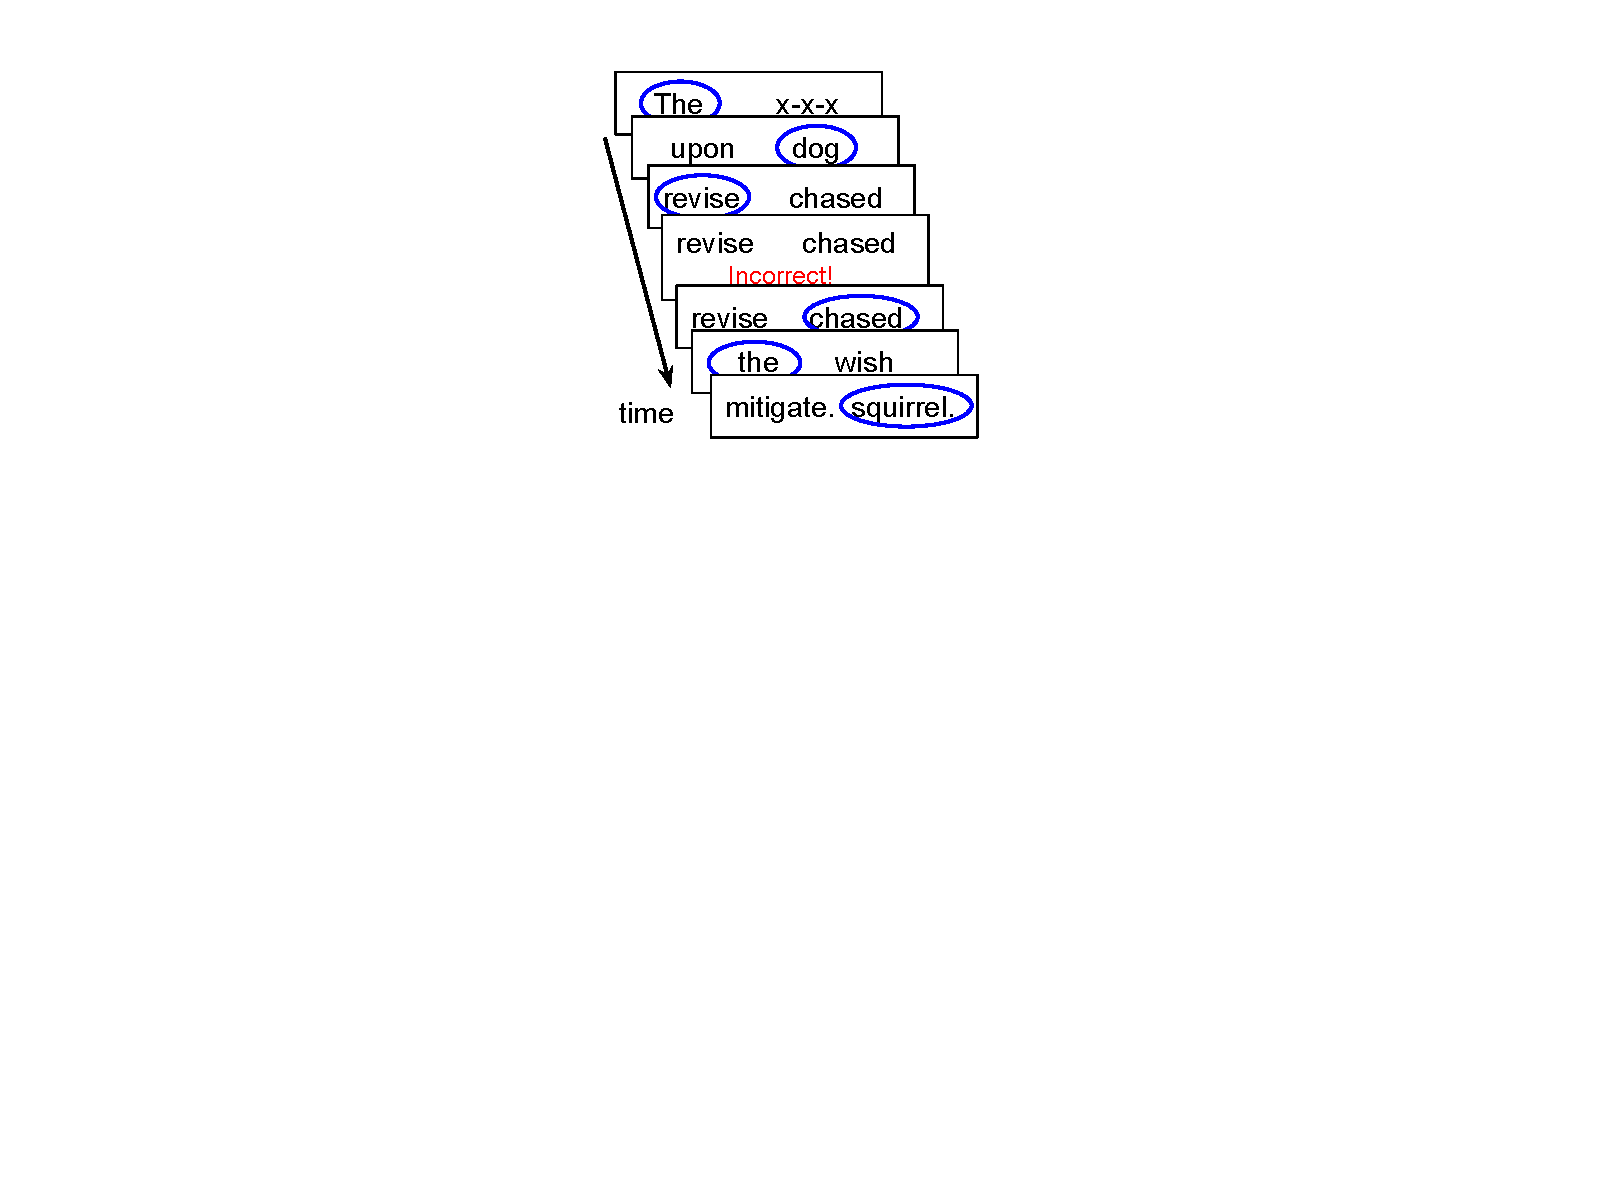
\includegraphics[clip, trim=9cm 12.5cm 10cm 1cm,width=.8\textwidth]{maze_diagram.pdf}\\} 
		\begin{small}
			Participants see two words at a time and try to select the correct word.  When the participant makes a mistake, they must correct it to continue. Blue circles indicate selected words.
			
		\end{small}
		
	\end{minipage}
	~~~
	\begin{minipage}{.5\textwidth}	
				\captionof{figure}{Accuracy versus RT}
		{\center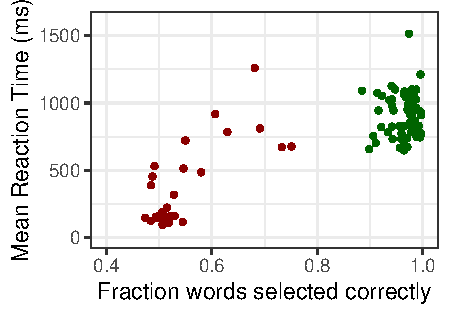
\includegraphics[width=\textwidth]{error.pdf}\\} 
		\begin{small}
			Correlation between participant's accuracy on the Maze task and RT. Participants with less than 80\% accuracy (in red) were excluded from analyses. 
			
		\end{small}
	\end{minipage}
\end{figure}
\begin{figure}
		\begin{minipage}{.5\textwidth}
		\captionof{figure}{Surprisal and RT\\
		}
		{\center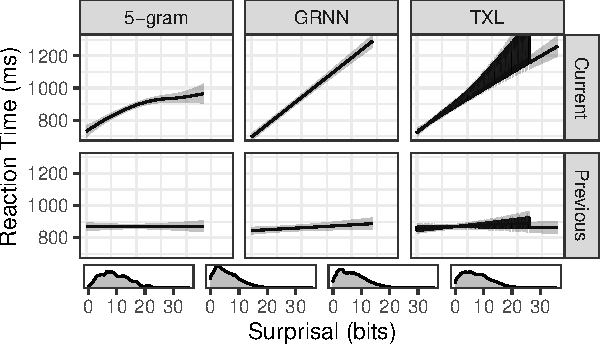
\includegraphics[width=\textwidth]{gam.pdf}\\} 
		\begin{small}
			Current word surprisal is linearly predictive of RT, but previous word surprisal is not predictive of RT.
			
		\end{small}
	\end{minipage}	
	~~~
\begin{minipage}{.5\textwidth}
	\captionof{figure}{Comprehension question accuracy}
	{\center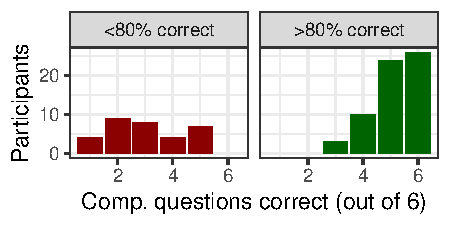
\includegraphics[width=\textwidth]{comp.pdf}\\} 
	\begin{small}
		Participants with high accuracy on the Maze task also perform well on comprehension questions. 
		
	\end{small}
\end{minipage}
	
\end{figure}

	\setlength{\tabcolsep}{3pt}
		\captionof{table}{Regression Coefficients}
\begin{small}%TODO do I even include p-values??
%\centering
\begin{tabular}{l|rlr|rlr|rlr}
	\hline
	&\multicolumn{3}{c|}{5-gram}&\multicolumn{3}{c|}{GRNN}&\multicolumn{3}{c}{TXL}\\
		 & Est & CI & $p$ & Est & CI & $p$ &Est & CI & $p$ \\ 
		 \hline
Intercept & 865.3 & [829.9, 902.9] & 0.00 & 871.1 & [837.9, 905.3] & 0.00 & 870.8 & [832.5, 907.8] & 0.00 \\ 
Surprisal & 11.7 & [9.3, 14.1] & 0.00 & 23.7 & [21, 26.5] & 0.00 & 18.5 & [16.1, 21.1] & 0.00 \\ 
Frequency & -2.9 & [-6.3, 0.5] & 0.10 & 2.9 & [-0.2, 6] & 0.06 & 0.4 & [-2.7, 3.5] & 0.79 \\ 
		Length & 20.5 & [15.4, 25.6] & 0.00 & 18.5 & [13.3, 23.7] & 0.00 & 21.4 & [16.2, 26.6] & 0.00 \\ 
		Surprisal:Length & -2.0 & [-3, -1] & 0.00 & -1.8 & [-2.7, -0.9] & 0.00 & -1.4 & [-2.2, -0.6] & 0.00 \\
		Freq:Length & -1.0 & [-2.5, 0.4] & 0.16 & -0.1 & [-1.2, 1] & 0.82 & 0.2 & [-0.9, 1.2] & 0.76 \\ 
		\hline
			Past Surprisal & 1.6 & [-0.5, 3.6] & 0.14 & 2.7 & [0.8, 4.5] & 0.00 & 0.8 & [-0.9, 2.5] & 0.40 \\ 
		Past Freq & 2.6 & [-0.1, 5.4] & 0.06 & 1.9 & [-0.2, 4.2] & 0.08 & 1.2 & [-1.1, 3.6] & 0.30 \\ 
		Past Length & -4.8 & [-9, -0.1] & 0.04 & -6.6 & [-10.9, -2.1] & 0.00 & -5.2 & [-9.3, -0.7] & 0.03 \\ 
				Past Surp:Length & -0.2 & [-1.2, 0.8] & 0.72 & -0.9 & [-1.7, -0.2] & 0.01 & -0.6 & [-1.3, 0.2] & 0.13 \\ 
		Past Freq:Length & -1.0 & [-2.3, 0.3] & 0.15 & -1.8 & [-2.9, -0.8] & 0.00 & -1.5 & [-2.6, -0.5] & 0.01 \\ 
	


		 
\hline
\end{tabular}
\vspace{.1em}

\end{small}
		\begin{small}
			Point estimates, credible intervals, and p-value equivalents. Surprisal was measured in bits, frequency in $log_2$ occurrences per billion words, and length in characters. All predictors were centered, and only single token words were included. Models were fit in BRMS with formula \textit{rt $\sim$ surprisal*length + freq*length + past\_surp*past\_length + past\_freq*past\_length +
			(surprisal*length + freq*length + past\_surp*past\_length + past\_freq*past\_length | participant)+(1|word\_id)}. Results shown for regression on pre-error data only.
		\end{small}

\vspace{.1em}
	\begin{small}{
			\noindent\textbf{References:}
			Boyce et al (2020). \textit{J Mem. Lang.} $\bullet$
			Dai et al (2019) arXiv:1901.02860 $\bullet$
			Forster et al (2009). \textit{Behav. Res. Methods} $\bullet$
			Futrell et al (2017). arXiv:1708.05763 $\bullet$
			Gulordava et al (2018).  \textit{NAACL-HLT 2018} $\bullet$
			Shain (2019). \textit{NAACL-HLT 2019} $\bullet$
			Sloggett et al (2020). \textit{CUNY 2020} $\bullet$
			Smith \& Levy (2013). \textit{Cognition} $\bullet$
			Witzel et al (2012).  \textit{J Psycholinguist Res.} 
		}
	\end{small}

\end{document}
